\chapter{Implementation}
\label{chap:impl}

\section{\Rzk{} Language Server and VS Code extesion}

In this section, we describe the implementation of the language server
and the VS Code extension for the \Rzk{} proof assistant.
The language server has direct access to the proof assistant internals,
including the typechecking algorithm and the internal abstract syntax representation,
and provides an interface conforming to the Language Server Protocol.
The VS Code extension then acts as a intermediary between the editor (VS Code)
and the language server, to bring the interactive capabilities to the user.

\subsection{Features}

% TODO: move this subsection to the requirements/design chapter?

We subject the language server to support the features specified below.

\subsubsection{Intuitive Interface and Syntax Highlighting.}

The VS Code extension introduces an intuitive interface that aligns with
the expectations of mathematicians and computer scientists.
Users benefit from clear and accessible navigation,
enabling efficient exploration of HoTT-based structures.
Furthermore, the extension provides syntax and semantic highlighting,
enhancing code readability, and facilitating error detection.

\begin{figure}
  \centering
  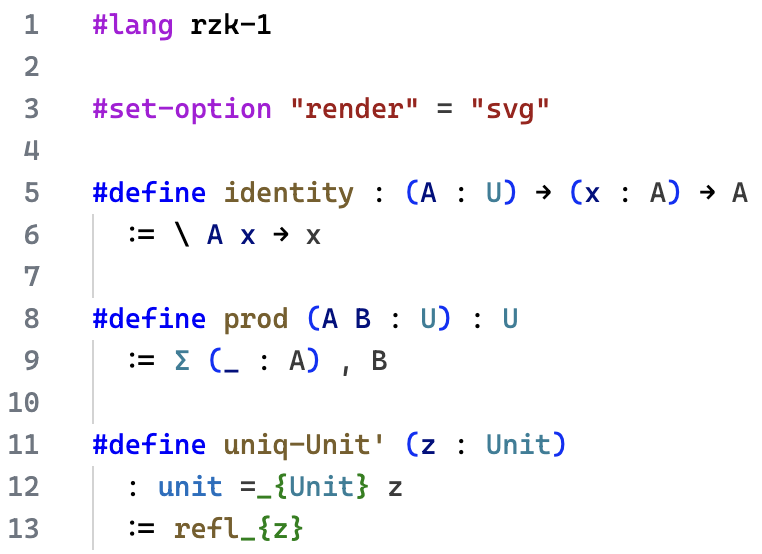
\includegraphics[width=0.7\textwidth]{figs/syntax-highlighting.png}
  \caption{Syntax/Semantic highlighting in VS Code.}
  \label{figure:syntax-highlighting}
\end{figure}

\subsubsection{Code Completion and Suggestions.}

\Rzk{}'s VS Code extension leverages the LSP to offer intelligent code completion
and context-aware suggestions. As users work with \Rzk{}, the extension assists
in writing code more efficiently by providing relevant suggestions, reducing
the likelihood of syntax errors, and accelerating the development process.

\begin{figure}
  \centering
  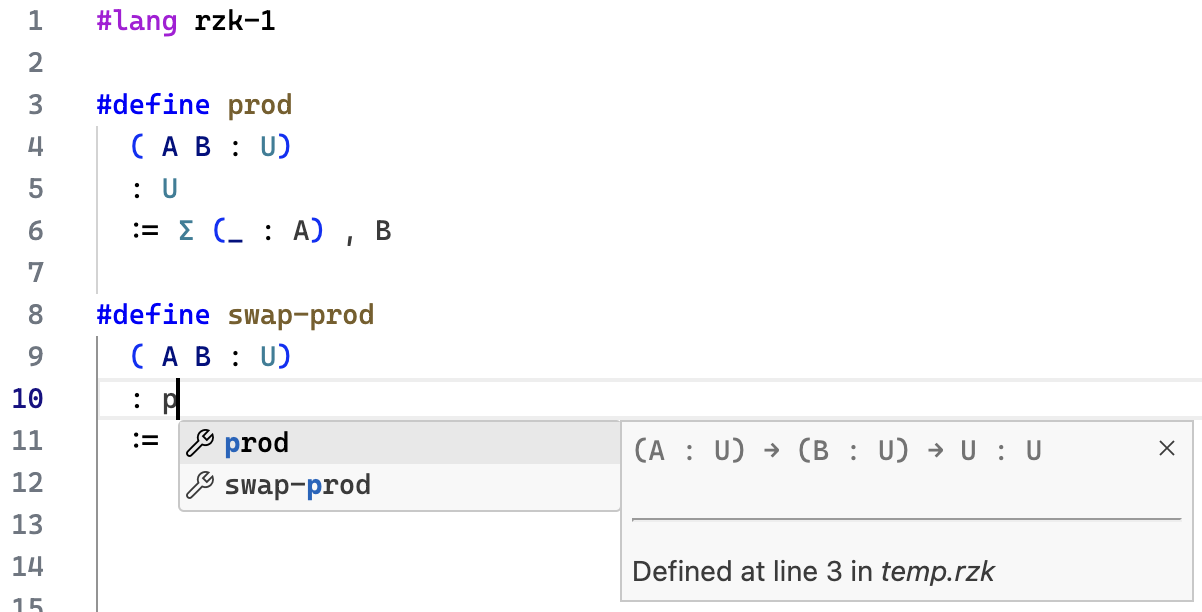
\includegraphics[width=0.7\textwidth]{figs/code-completions.png}
  \caption{Code completions in VS Code.}
  \label{figure:code-completions}
\end{figure}

\subsubsection{Real-time Error Checking.}

One of the extension's notable strengths lies in its ability to perform real-time error checking.
As users input and modify code, the language server continuously analyzes it,
reporting back any type errors or other issues with the proof.
This proactive error checking mechanism empowers users to identify and rectify issues promptly,
fostering the creation of mathematically sound programs.

\begin{figure}
  \centering
  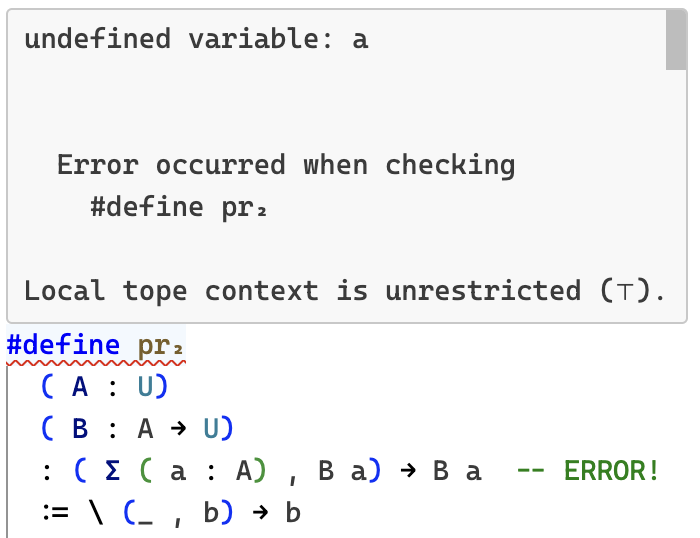
\includegraphics[width=0.7\textwidth]{figs/diagnostic-message.png}
  \caption{An error diagnostic message in VS Code.}
  \label{figure:diagnostic-message}
\end{figure}

\subsection{VS Code extension}

To bring about these features to the users, a thin wrapper around the language server in the form of a VS Code extension is necessary.
Additionally, the extension manages the installation of the language server itself on all major operating systems (Windows, macOS, and Ubuntu)
powered by pre-built binaries attached to releases on GitHub,
in addition to facilitating building the language server from source on platforms
for which pre-built binaries are not available.
The source code of the extension is available on the GitHub repository\footnote{
  \url{https://github.com/rzk-lang/vscode-rzk}},
and the extension itself is available on the Visual Studio Marketplace\footnote{
  \url{https://marketplace.visualstudio.com/items?itemName=NikolaiKudasovfizruk.rzk-1-experimental-highlighting}}.
and on the Open VSX registry\footnote{
  \url{https://open-vsx.org/extension/NikolaiKudasovfizruk/rzk-1-experimental-highlighting}},
as well as a pre-built binary on the GitHub releases page\footnote{
  \url{https://github.com/rzk-lang/vscode-rzk/releases}}.

\subsubsection{Installation and Activation}

Once the extension is activated, it checks if the \Rzk{} executable is available on the system's
\texttt{PATH} and if not, checks if it was previously downloaded to the extension's local storage directory.
If neither are available, it prompts the user to download the latest compatible binary from the GitHub
releases page and saves it in the local storage directory.
The user can override this behavior by specifying a custom path to the language server binary.

\begin{listing}
  \begin{minted}{typescript}
function locateRzk(context: vscode.ExtensionContext) {
  let path = vscode.workspace.getConfiguration().get<string>('rzk.path') ?? '';
  // Probe 1 - extension settings
  if (path) {
    const result = spawnSync(path, ['version']);
    if (result.status === 0) {
      return path;
    } else {
      output.appendLine(
        'The configured `rzk.path` option does not point to a valid rzk executable'
      );
    }
  }

  // Probe 2 - global PATH
  const binExtension = process.platform === 'win32' ? '.exe' : '';
  path = 'rzk' + binExtension;
  let result = spawnSync(path, ['version']);
  if (result.status === 0) {
    return path;
  } else {
    output.appendLine('Cannot find rzk globally');
  }

  // Probe 3 - extension storage bin folder
  path = vscode.Uri.joinPath(
    context.globalStorageUri,
    'bin',
    'rzk' + binExtension
  ).fsPath;
  result = spawnSync(path, ['version']);
  if (result.status === 0) { return path; }

  return null;
}
  \end{minted}
  \caption{The function responsible for finding where \Rzk{} is installed}
  \label{code:locate-rzk}
\end{listing}

To download a pre-built binary of \Rzk{}, the extension queries the available releases on the
GitHub repository and finds the latest release compatible with the installed version of the extension.
Compatibility is determined by defining a semver \cite{Preston2013semantic} range in the extension's source code,
which is then used to filter the releases and find the latest one that satisfies the range.

\begin{listing}
  \begin{minted}{typescript}
import semver from 'semver';
import type { RestEndpointMethodTypes } from '@octokit/rest';

/** In semver range format */
const supportedRzkVersions = '>=0.6.0 <1.0.0';

type GitHubRelease =
  RestEndpointMethodTypes['repos']['listReleases']['response']['data'][number];

/**
 * Checks whether the given rzk version is compatible with the extension
 * @param version A version string, e.g. "1.3.2" or "v0.4.1.1"
 */
export function isCompatibleVersion(version: string) {
  return semver.satisfies(semver.coerce(version) ?? '', supportedRzkVersions);
}
  \end{minted}
  \caption{Version compatibility check in the VS Code extension.}
  \label{code:ext-version}
\end{listing}

Then, the extension downloads the binary using Octokit SDK and extracts the tar archive to the local storage directory.

After that, the extension simply starts the language server in a separate process and establishes a connection to it,
and the rest is handled by VS Code and the language server.

\subsubsection{Configuration}

The extension provides configuration options to the user to customize the behavior of the extension.
The user can specify the path to the \Rzk{} executable, which is useful for users who have the executable installed in a non-standard location, as well as for testing purposes.
The user can also enable or disable the formatting feature and choose whether to receive pre-release versions of \Rzk{}.

\begin{figure}
  \centering
  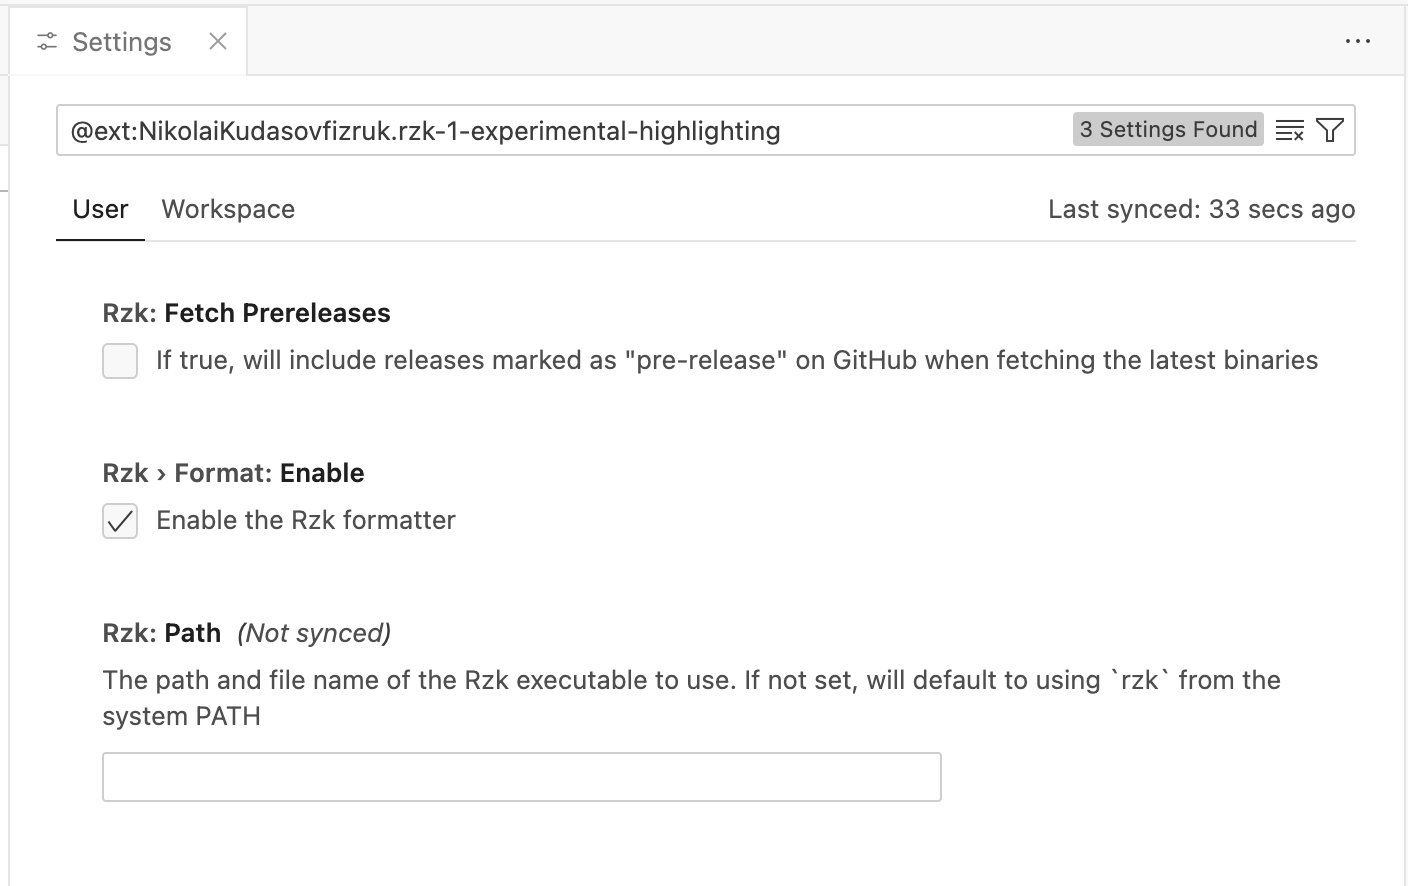
\includegraphics[width=0.8\textwidth]{figs/rzk-vscode-settings.png}
  \caption{The extension configuration section in VS Code.}
  \label{figure:vscode-settings}
\end{figure}

This is achieved using the configuration\footnote{
  \url{https://code.visualstudio.com/api/references/contribution-points\#contributes.configuration}}
field in \texttt{package.json}

\subsection{\Rzk{} Language Server}

At the core of the \Rzk{} tool suite is the language server that powers all the editor features that make it pleasant to develop proofs in \Rzk{}. In particular, it currently supports semantic highlighting, diagnostic messages, and text completion. Additionally, progress reporting for long-running processes (such as type-checking for large projects) is currently under work.

For the first versions of the language server, it is shipped as part of the \Rzk{} proof assistant itself under a different subcommand, but it is planned to decouple both components and have the language server depend on the core library. They are implemented in the Haskell programming language using the \texttt{lsp}\footnote{\url{https://hackage.haskell.org/package/lsp}} package.

This entry point is made available to the user as a separate subcommand, \texttt{rzk lsp},
which starts the language server and listens for incoming connections from the editor.
It defines the handlers for the LSP messages and initializes the server with the necessary configuration
for synchronizing between the files in the editor and the language server.

\begin{listing}
  \begin{minted}{haskell}
handlers :: Handlers LSP
handlers =
  mconcat
    [ notificationHandler SMethod_Initialized $ const typecheckFromConfigFile
    -- Empty handlers omitted for brevity
    , notificationHandler SMethod_WorkspaceDidChangeWatchedFiles handleFilesChanged
    , requestHandler SMethod_TextDocumentCompletion provideCompletions
    , requestHandler SMethod_TextDocumentSemanticTokensFull provideSemanticTokens
    , requestHandler SMethod_TextDocumentFormatting formatDocument
    ]

syncOptions :: TextDocumentSyncOptions
syncOptions = TextDocumentSyncOptions
  { _openClose         = Just True
  , _change            = Just TextDocumentSyncKind_Full
  , _willSave          = Just False
  , _willSaveWaitUntil = Just False
  , _save              = Just $ InR $ SaveOptions { _includeText = Just True }
  }

runLsp :: IO Int
runLsp = do
  rzkEnv <- defaultRzkEnv
  runServer $
    ServerDefinition
      { configSection = "rzk"
      , parseConfig = \_oldConfig newObject -> case fromJSON newObject of
          Error err         -> Left $ T.pack err
          Success rzkConfig -> Right rzkConfig
      , onConfigChange = const $ pure ()
      , doInitialize = const . pure . Right
      , staticHandlers = const handlers
      , interpretHandler = \env -> Iso (flip runReaderT rzkEnv . runLspT env) liftIO
      , options = defaultOptions { optTextDocumentSync = Just syncOptions }
      , defaultConfig = def :: ServerConfig
      }
  \end{minted}
  \caption{Initialization of the language server}
  \label{code:server-init}
\end{listing}

It is also worth mentioning that the language server is designed to be compatible
with any other editor that supports LSP, not just VS Code.
In particular, users have reported success in integrating it with the NeoVim editor,
and it is planned to be tested with other editors as well.

The language server currently supports the features outlined in the following sections, with more features planned for the future.

\subsubsection{Diagnostics Reporting}

Every time the user saves a file that is part of a formalization project, the language server runs the typechecker
on the project and reports any errors or warnings that it finds, caching the results to speed up future typechecks.
The errors and warnings are sent as diagnostic messages via the LSP protocol to the editor,
which then displays them in the editor's interface.
This feature is crucial for the users to be able to quickly identify and fix any errors in their proofs.
These messages are displayed on the location in the file where the error occurred,
and contain a useful message that explains what went wrong with all the necessary context.

The process starts by looking for an \texttt{rzk.yaml} configuration file in the project directory,
which contains information about which files are included in the project.
Then, the language server parses the modified files, and if they parse successfully,
runs the typechecker on then and collects the type errors.
Finally, it sends the diagnostic messages (both parsing and type errors) to the editor,
which then displays them to the user.
An example of such a diagnostic message can be seen in Figure \ref{figure:diagnostic-message}.

Since this process is computationally expensive, the language server caches the results of the typechecker
and only re-runs it on the files that have changed since the last typecheck.
Ideally, \Rzk{} would support incremental parsing and have a more granular and efficient check
on what declarations exactly have changed, but this is currently not implemented.

\subsubsection{Text Completion}

The language server also provides text completion suggestions to the user as they type.
These suggestions are context-aware and are based on the current cursor position in the file.
They include previously defined proof identifiers, their types, and their definition locations.

To provide the text completions items, the declarations that successfully typechecked are
retrieved from the cache, which also includes information about their types and definition location.
Then, the language server filters these declarations based on the current cursor position
and sends them to the editor as completion items.
This process (with irrelevant definitions omitted for brevity) can be seen in listing \ref{code:completions}.

\begin{listing}
  \begin{minted}{haskell}
provideCompletions :: Handler LSP 'Method_TextDocumentCompletion
provideCompletions req res = do
  root <- getRootPath
  let rootDir = fromMaybe "/" root
  cachedModules <- getCachedTypecheckedModules
  let currentFile = fromMaybe "" $ uriToFilePath $ req ^. params . textDocument . uri
  -- Take all the modules up to and including the currently open one
  let modules = map ignoreErrors $ takeWhileInc ((/= currentFile) . fst) cachedModules
        where
          ignoreErrors (path, RzkCachedModule{..}) = (path, cachedModuleDecls)
          takeWhileInc _ [] = []
          takeWhileInc p (x:xs)
            | p x       = x : takeWhileInc p xs
            | otherwise = [x]
  let items = concatMap (declsToItems rootDir) modules
  res $ Right $ InL items
  \end{minted}
  \caption{Completions providing function in the language server}
  \label{code:completions}
\end{listing}

An example for these completions items can be seen in Figure \ref{figure:code-completions}.

\subsubsection{Semantic Highlighting}

Another feature that the language server provides is semantic highlighting, which colors different parts of the code
based on their meaning.
This differs from syntax highlighting in that it is smarter and can use more information in determining a token's type (and hence color),
This is because it uses information from the parser, and not just from the lexer.
It can also use additional information from the typechecker to determine the type of a token,
but this is currently not implemented since it was not deemed necessary.

A (simplified) snippet of the code implementing semantic highlighting can be seen in listing \ref{code:semantic-highlighting},
and an example of semantic highlighting in the editor can be seen in Figure \ref{figure:syntax-highlighting}.

\begin{listing}
  \begin{minted}{haskell}
tokenizeTerm :: Term -> [SemanticTokenAbsolute]
tokenizeTerm term = case term of
  Universe{}           -> mkToken term SemanticTokenTypes_Class [defLib]
  UniverseCube{}       -> mkToken term SemanticTokenTypes_Class [defLib]
  UniverseTope{}       -> mkToken term SemanticTokenTypes_Class [defLib]

  CubeUnit{}           -> mkToken term SemanticTokenTypes_Enum [defLib]
  CubeUnitStar{}       -> mkToken term SemanticTokenTypes_EnumMember [defLib]
  ASCII_CubeUnitStar{} -> mkToken term SemanticTokenTypes_EnumMember [defLib]

  Cube2{}              -> mkToken term SemanticTokenTypes_Enum [defLib]
  Cube2_0{}            -> mkToken term SemanticTokenTypes_EnumMember [defLib]
  where
    defLib = SemanticTokenModifiers_DefaultLibrary
  \end{minted}
  \caption{Sample of the tokenizing function for terms}
  \label{code:semantic-highlighting}
\end{listing}

\subsubsection{Formatting}

The language server also provides a formatting feature that allows the user to format their code according to a predefined style.
This is useful for keeping the codebase consistent and readable, and is especially useful when working in a team.
The formatter catches common style issues such as indentation, spacing, and line breaks,
and automatically fixes them according to the predefined style.

The formatter is implemented in the core part of \Rzk{} itself.
A separate CLI subcommand is available to expose this feature outside of the language server as well.

The formatter uses the tokens produced from the lexical analysis step and attempts to find
common style issues such as missing line breaks, incorrect indentation, and extra spaces.
The approach of using the tokens was chosen because the parser does not produce a Concrete Syntax Tree
that can be used for pretty-printing.
This approach also allows for more flexibility in the coding style, while enforcing a few best practices.
These best practices are outlined in the sHoTT repository's style guide\footnote{
  \url{https://rzk-lang.github.io/sHoTT/STYLEGUIDE/}}.

An example of the formatting function can be seen in listing \ref{code:formatting}.
Figure \ref{figure:formatting} shows an example of the formatting feature in action.

\begin{listing}
  \begin{minted}{haskell}
formatTextEdits :: String -> [FormattingEdit]
formatTextEdits contents =
  case resolveLayout True (tokens rzkBlocks) of
    Left _err -> [] -- TODO: log error (in a CLI and LSP friendly way)
    Right allToks -> go (initialState {allTokens = allToks}) allToks
  where
    -- Line break before := and one space after
    go s (Token ":=" line col : tks)
      = edits ++ go s tks
      where
        lineContent = contentLines line
        isFirstNonSpaceChar = all (== ' ') (take (col - 1) lineContent)
        spacesAfter = length $ takeWhile (== ' ') (drop (col + 1) lineContent)
        spacesBefore = length $ takeWhile (== ' ') (reverse $ take (col - 1) lineContent)
        edits = map snd $ filter fst
            -- Ensure line break before `:=`
          [ (not isFirstNonSpaceChar, FormattingEdit line (col - spacesBefore) line col "\n  ")
            -- Ensure 2 spaces before `:=` (if already on a new line)
          , (isFirstNonSpaceChar && spacesBefore /= 2,
              FormattingEdit line 1 line col "  ")
            -- Ensure exactly one space after
          , (length lineContent > col + 2 && spacesAfter /= 1,
              FormattingEdit line (col + 2) line (col + 2 + spacesAfter) " ")
          ]
    -- Remove any space before the closing paren
    go s (Token ")" line col : tks)
      = edits ++ go (decParensDepth s) tks
      where
        lineContent = contentLines line
        isFirstNonSpaceChar = all (== ' ') (take (col - 1) lineContent)
        spacesBefore = length $ takeWhile (== ' ') (reverse $ take (col - 1) lineContent)
        edits = map snd $ filter fst
          [ (not isFirstNonSpaceChar && spacesBefore > 0,
              FormattingEdit line (col - spacesBefore) line col "")
          ]
    -- Other patterns ...
  \end{minted}
  \caption{Part of the formatting function}
  \label{code:formatting}
\end{listing}

\begin{figure}
  \centering
  \begin{minipage}{0.55\textwidth}
    \centering
    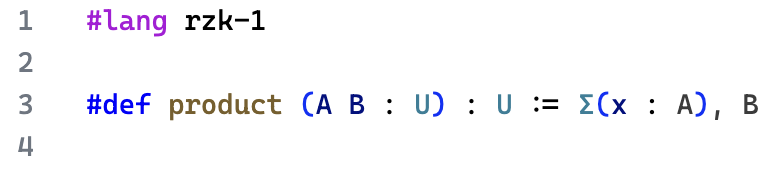
\includegraphics[width=\textwidth]{figs/formatting-before.png}
  \end{minipage}\hfill
  \begin{minipage}{0.35\textwidth}
    \centering
    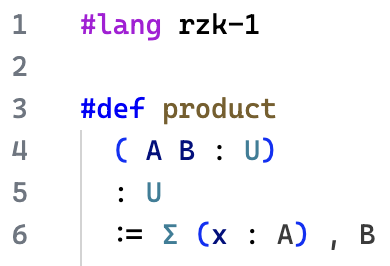
\includegraphics[width=\textwidth]{figs/formatting-after.png}
  \end{minipage}
  \caption{Before and after formatting a definition}
  \label{figure:formatting}
\end{figure}

\section{Satellite Tools}

In addition to the VS Code extension and the lagnuage server, work on this project also
involved the development of several satellite tools that are used along with \Rzk{}
for a more complete development experience.
The most noteworthy of these tools are a plugin for the MkDocs static site generator\footnote{
  \url{https://www.mkdocs.org/}}
and a GitHub Action that can be used to run \Rzk{} in Continuous Integration (CI) pipelines.

\subsection{MkDocs Plugin}

MkDocs is a static site generator that is commonly used to generate documentation websites.
Sources are written in Markdown, which is convenient for \Rzk{} in particular since the \Rzk{}
proofs can be written in the Literate Programming style, where the proofs are interspersed with
explanatory text, for which the Markdown format is supported in \Rzk{}.

The MkDocs plugin for \Rzk{} is a Python package that provides a plugin for MkDocs that can render
tope diagrams in the documentation.
It does so by running the \Rzk{} executable on the Markdown files and extracting any SVG
output in the process's standard output stream.
The figures are then mapped to the definitions that produced them and are inserted into the
Markdown files as SVG diagrams right next to the definitions.
It also adds some CSS code to the generated HTML to scale up the diagram on hover.

An example of the rendered figure in the generated documentation can be seen in Figure \ref{figure:svg-rendering}.
\begin{figure}
  \centering
  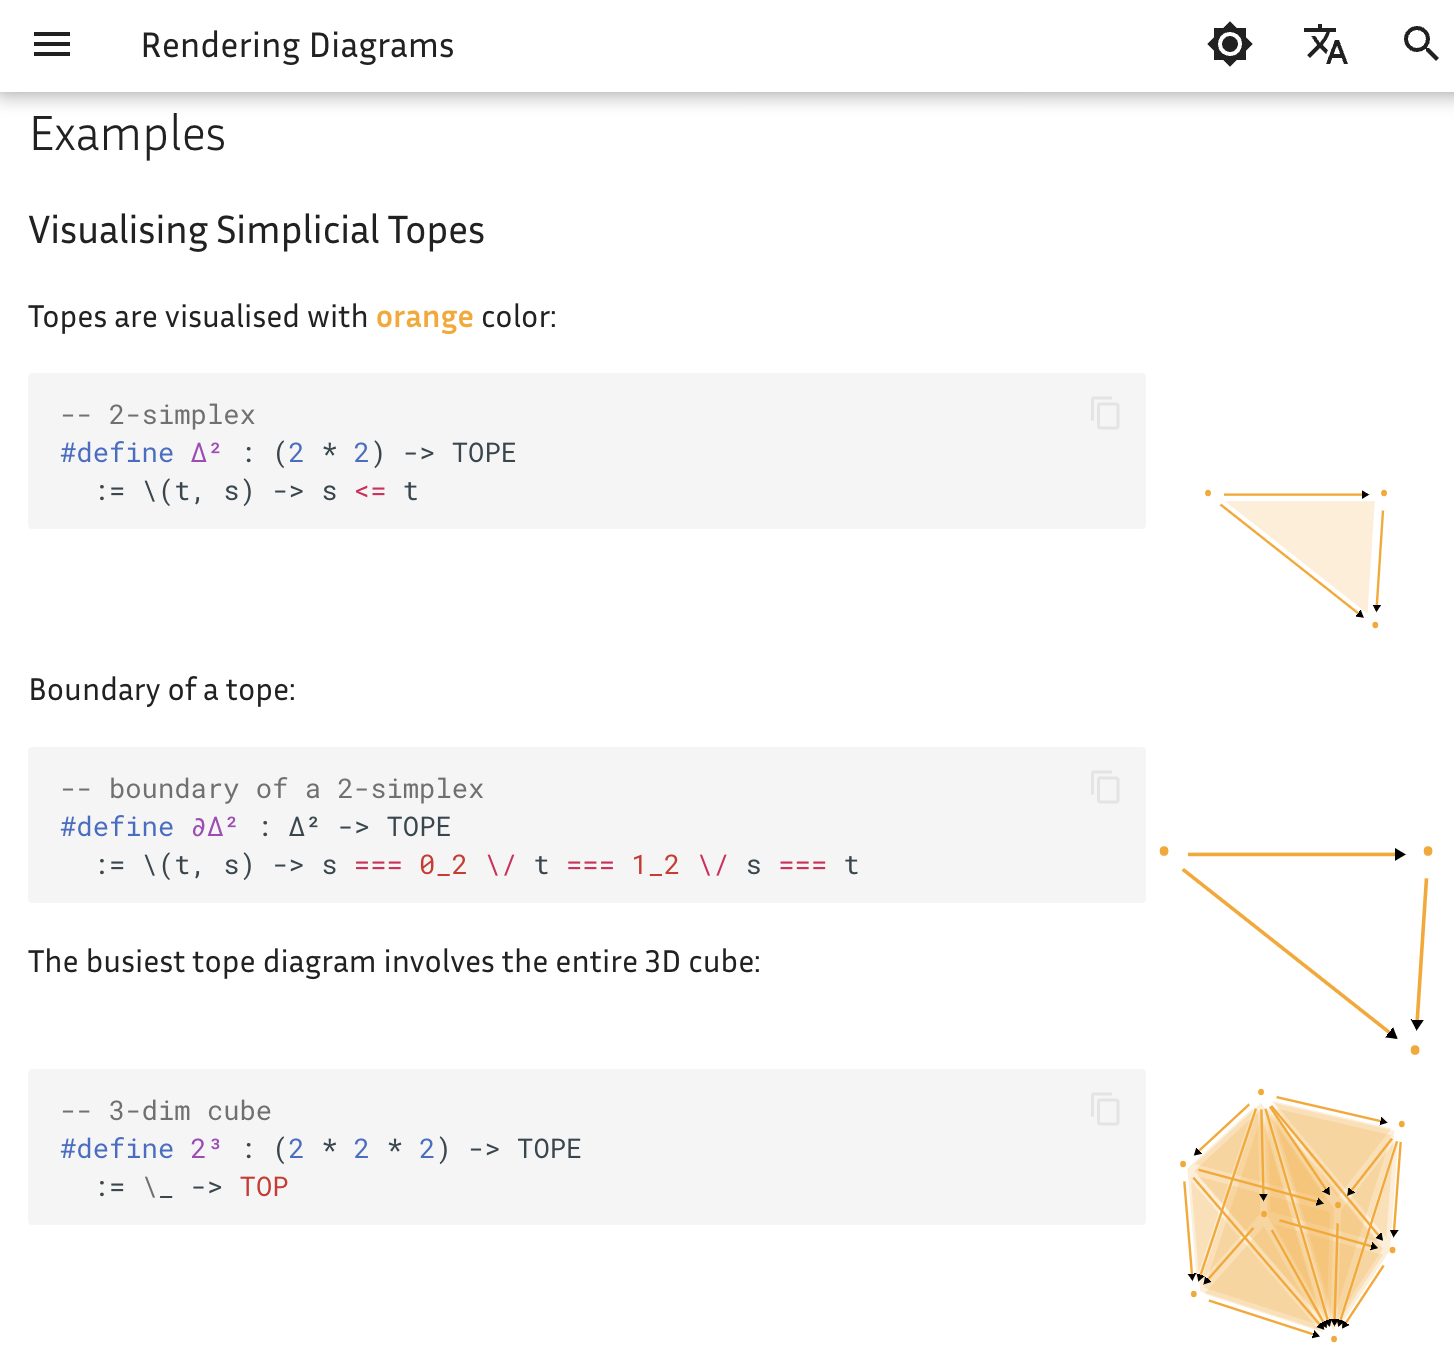
\includegraphics[width=0.8\textwidth]{figs/svg-rendering.png}
  \caption{The rendered diagrams inserted next to their definitions.}
  \label{figure:svg-rendering}
\end{figure}

Another minor feature the plugin supports is generating hyperlinks for all definitions on a page
so that the user can easily navigate to the definition's location by clicking on the hyperlink.
The definition's name itself becomes a hyperlink that leads to the its location in the page.

Both of these featues are configurable in the \texttt{mkdocs.yml} configuration file,
where the user can specify the path to the \Rzk{} executable, whether to generate SVGs,
and whether to generate hyperlinks or not.
An example of such configuration can be seen in listing \ref{code:mkdocs-config}.

\begin{listing}
  \begin{minted}{yaml}
plugins:
  - rzk:
      render_svg: true
      anchor_definitions: true
  \end{minted}
  \caption{Plugin section of the \texttt{mkdocs.yml} configuration file of \Rzk{}'s documentation}
  \label{code:mkdocs-config}
\end{listing}

The plugin is available on the Python Package Index\footnote{
  \url{https://pypi.org/project/mkdocs-plugin-rzk/}},

\subsection{GitHub Action}

GitHub Actions \footnote{\url{https://github.com/features/actions}} is the CI workflow automation
tool provided by GitHub that allows users to define workflows in YAML files that can be run
on every push to the repository, on pull requests, or on other events.

For formalization projects using \Rzk{}, it is important to be able to check the proofs
for correctness on every push or pull request to the repository, to ensure that no incorrect
formalizations are merged into the main branch.
To that end, a GitHub Action was developed that can be used to run the \Rzk{} executable
on the project files and check them for correctness.
This adds a status check to the pull requests that shows whether the proofs typecheck or not,
and possibly prevents merging if they do not.
The status check is displayed next to the commit that triggerred the CI with either
a green checkmark if it typechecks or a red cross if it doesn't, making the status easily visible
to proof developers.
The full output of the typechecker is also displayed in the GitHub Actions logs, so that the user
can see what went wrong and fix it.

Using the GitHub Action is as simple as adding a step to the workflow file with the snippet
in listing \ref{code:rzk-action-step}.
A full example of a workflow file can also be seen in listing \ref{code:rzk-action-full}.

\begin{listing}
  \begin{minted}{yaml}
- name: Typecheck Rzk files
  uses: rzk-lang/rzk-action@v1
  with:
    rzk-version: latest
  \end{minted}
  \caption{GitHub Actions step for checking an \Rzk{} project}
  \label{code:rzk-action-step}
\end{listing}

\begin{listing}
  \begin{minted}{yaml}
name: Typecheck with latest Rzk

# Controls when the workflow will run
on:
  # Triggers the workflow on pull requests to the main branch
  pull_request:
    branches:
      - main

jobs:
  check:
    runs-on: ubuntu-latest
    name: Check formalisations
    steps:
      - uses: actions/checkout@v3

      - name: Typecheck Rzk files
        uses: rzk-lang/rzk-action@v1.2.0
        with:
          rzk-version: v0.7.1
          files: src/**/*.rzk.md
          check-formatting: true
  \end{minted}
  \caption{Full GitHub Actions workflow file for checking an \Rzk{} project}
  \label{code:rzk-action-full}
\end{listing}
